% =====================================================================
%  Structure-informed robust weighting for photometric visual servoing
%  under occlusion: a pre-registered simulation study
%
%  Draft for Robotics and Autonomous Systems (Elsevier, elsarticle).
%  Every number in this manuscript is taken from the committed campaign
%  outputs (RESULTS.md, confirmatory/, replication/, sweep/); figures are
%  regenerated by paper/make_figures.py.
%  Items to complete before submission are marked TODO.
% =====================================================================
\documentclass[preprint,12pt]{elsarticle}

\usepackage[T1]{fontenc}
\usepackage{lmodern}
\usepackage{amsmath,amssymb,amsthm}
\usepackage{graphicx}
\usepackage{booktabs}
\usepackage{array}
\usepackage{xcolor}
\usepackage{microtype}
\usepackage[hidelinks]{hyperref}

\newtheorem{proposition}{Proposition}
\newtheorem{lemma}{Lemma}
\newtheorem{corollary}{Corollary}
\theoremstyle{remark}
\newtheorem{remark}{Remark}

\newcommand{\Lh}{\widehat{\mathbf{L}}}
\newcommand{\W}{\mathbf{W}}
\newcommand{\HW}{\mathbf{H}_{\mathbf{W}}}
\newcommand{\KW}{\mathbf{K}_{\mathbf{W}}}
\newcommand{\e}{\mathbf{e}}
\newcommand{\s}{\mathbf{s}}
\newcommand{\vc}{\mathbf{v}}
\newcommand{\dr}{\delta\mathbf{r}}
\newcommand{\Gb}{\bar{G}}
\newcommand{\med}{\operatorname{med}}
\newcommand{\tr}{\operatorname{tr}}
\newcommand{\diag}{\operatorname{diag}}
\newcommand{\todo}[1]{\textcolor{red}{[TODO: #1]}}

\journal{Robotics and Autonomous Systems}

\begin{document}

\begin{frontmatter}

\title{Structure-informed robust weighting for photometric visual servoing
under occlusion: a pre-registered simulation study}

\author[inst1]{Selma Boutiba\corref{cor1}}
\ead{TODO-institutional-email@example.org}
\cortext[cor1]{Corresponding author.}
\author[inst1]{\todo{co-authors and supervisors}}
\affiliation[inst1]{organization={\todo{laboratory, university}},
            city={\todo{city}},
            country={\todo{country}}}

\begin{abstract}
Direct visual servoing feeds every pixel into the control law, so a partial
occlusion biases the commanded velocity unless the corrupted measurements are
down-weighted. We study a structure-informed robust weighting for Hermite
photometric visual servoing, which normalises each residual by a local
Gauss--Hermite gradient magnitude of the current image before applying Tukey's
biweight. We show that, when the interaction matrix is computed from the
current image, measurements in untextured regions have zero interaction rows,
so their weights cannot affect the control. We also give a sufficient
condition for local convergence under arbitrary time-varying weights. A
pre-registered simulation study of 1\,792 runs (32 initial poses, four occluder
appearances, occluded fractions of 7.5--45\,\%, two textures) compares the
weighting with Tukey weighting, a structure-penalising weighting and no
weighting. With the desired-image interaction matrix and a budget of 600
iterations, the structure-informed weighting reduces the camera-centre error of
Tukey weighting by a third (median ratio 0.66, 95\,\% CI 0.60--0.73,
Holm-adjusted $p=4.2\times10^{-7}$). The advantage is partly one of speed and
shrinks as the budget grows. Robustness to large occluders depends on how the
weighting is paired with the interaction matrix. With the desired-image matrix,
the structure-informed weighting converges from 27--30 of 32 poses up to
45\,\% occlusion while Tukey weighting fails from every pose; with the
current-image matrix the ordering reverses. On a second texture, Tukey
weighting converges from every pose to a biased equilibrium 128--175\,mm from
the target, which the structure-informed weighting avoids.
\end{abstract}

\begin{keyword}
Visual servoing \sep photometric visual servoing \sep robust estimation \sep
M-estimators \sep occlusion \sep Gauss--Hermite filters \sep pre-registration
\end{keyword}

\end{frontmatter}

% =====================================================================
\section{Introduction}
\label{sec:intro}

Photometric, or direct, visual servoing uses the image intensities themselves
as visual features~\cite{collewet2008setfree,collewet2011photometric}. It
dispenses with feature extraction, matching and tracking, and it reaches a
positioning accuracy that geometric features rarely match, because every pixel
contributes to the control law. The same property is its weakness: a region
of the image that does not obey the model of the scene---an occluder, a
specular highlight, a moving object---contributes as much as any other region,
and it biases the commanded velocity in proportion to its size and contrast.
Alternatives to raw intensities, such as mutual information~\cite{dame2011mutual},
photometric Gaussian mixtures~\cite{crombez2019pgm}, photometric
moments~\cite{bakthavatchalam2018moments} and multi-scale Gauss--Hermite filter
responses~\cite{herpvs}, change the representation but not this property.

The established remedy is robust estimation: each measurement receives a weight
computed by an M-estimator from the magnitude of its residual, and the weights
enter the control law~\cite{comport2006robust,malis2006robust}. Such a weighting
is \emph{structure-blind}: it judges a measurement by its residual alone. Early
in the servo, when the pose error is large, the residuals are large wherever
the image is textured, and a residual-based estimator rejects valid,
informative measurements together with the occluded ones. Direct visual
odometry addresses the same heteroscedasticity by weighting residuals with a
function of the image gradient~\cite{engel2014lsd,engel2018dso}. In DSO the
weight decreases with the gradient magnitude~\cite{engel2018dso}. The
structure-informed weighting studied here does the opposite: it normalises
each residual by a local gradient magnitude computed with the first-order
Gauss--Hermite kernels of the servoing scheme, so that a large residual at a
strongly textured position is treated as expected and a residual at an
untextured position as suspect. In the terminology of robust regression it is
a Schweppe-type generalised M-estimator~\cite{handschin1975bad,hampel1986robust}
whose design function reverses the usual bounded-influence direction.

Three questions are open. The first is \emph{where} a weighting can act. The
interaction matrix of a photometric feature is proportional to the image
gradient. When it is computed from the current image, as in many
implementations, measurements in a region that is uniform in the current image
have zero interaction rows, and no weight assigned to them can change the
control. When it is computed from the desired image, the same measurements have
non-zero rows. The choice between the two matrices is usually discussed in
terms of the convergence domain~\cite{chaumette2006vs1,malis2004esm}; its
consequence for robust weighting has not, to our knowledge, been analysed.
The second question is whether structure-informed weighting improves the final
accuracy, the convergence or both, and by how much. Evidence for robust
photometric servoing commonly rests on a few runs from one or two initial
poses, which cannot separate an effect from the variation between poses. The
third is how the competing weightings break down as the occluded fraction of
the image grows.

This paper makes three contributions.
\begin{enumerate}
\item An analysis of the weighted Levenberg--Marquardt photometric control
  law (Section~\ref{sec:analysis}): weights on measurements that are uniform in
  the current image are inert when the interaction matrix is taken from the
  current image (Proposition~\ref{prop:inert}); local convergence holds for
  any time-varying weight sequence under a rank condition that can be checked
  online (Proposition~\ref{prop:reweighting}); and the error-proportional gain
  of the scheme yields algebraic rather than geometric convergence on an
  unoccluded scene (Proposition~\ref{prop:rate}).
\item A pre-registered simulation study of 1\,792 runs
  (Section~\ref{sec:protocol}). The hypotheses, the primary tests, the
  multiple-comparison correction and the decision rule were committed to a
  version-controlled repository before the data were collected. The study
  comprises a confirmatory campaign (four weightings, two interaction
  matrices, four occluder appearances, 32 initial poses), a replication on a
  second texture and a sweep of the occluded fraction.
\item An account of when each weighting fails (Section~\ref{sec:results}).
  Tukey weighting retains occluded measurements whose residual happens to be
  small, which biases the equilibrium or causes divergence once the
  interaction matrix gives those measurements non-zero rows. The
  structure-informed weighting rejects an occluder by the absence of
  structure rather than by the size of its residual, but with the
  current-image matrix it fails late, along the weakly observable direction of
  a planar target. Its accuracy advantage at a fixed iteration budget shrinks as
  the budget grows, which the pre-registered outcome did not anticipate.
\end{enumerate}
Section~\ref{sec:related} reviews related work, Section~\ref{sec:setting}
states the servoing scheme, Section~\ref{sec:weightings} defines the
weightings compared, Section~\ref{sec:discussion} discusses the findings and
their limits, and Section~\ref{sec:conclusion} concludes.

% =====================================================================
\section{Related work}
\label{sec:related}

\paragraph{Direct visual servoing}
Photometric visual servoing~\cite{collewet2008setfree,collewet2011photometric}
regulates the difference between the current and desired images using the
interaction matrix of the luminance, derived from the brightness-constancy
assumption, and a Levenberg--Marquardt control law~\cite{marquardt1963}.
Subsequent work changed the feature to enlarge the convergence domain or to
gain robustness: mutual information~\cite{dame2011mutual}, which tolerates
occlusions and illumination changes through its statistical formulation;
photometric Gaussian mixtures~\cite{crombez2019pgm}; and photometric
moments~\cite{bakthavatchalam2018moments}. The scheme studied here,
Hermite photometric visual servoing (HER-PVS)~\cite{herpvs}, uses as features
the responses of summed Gauss--Hermite kernels~\cite{martens1990hermite} at four
scales. Its interaction matrix is obtained by filtering the luminance
interaction matrix with the same kernels.

\paragraph{Robust weighting in visual servoing}
Comport et al.~\cite{comport2006robust} introduced M-estimation into
image-based visual servoing: a diagonal weight matrix computed by
iteratively reweighted least squares multiplies both the error and the
interaction matrix, and the stability of the resulting law is discussed for
weights that vary slowly. Malis and Marchand~\cite{malis2006robust} compared
robust estimators for real-time robot vision. In these works the weights depend
on the residual alone. The interaction matrix used by the controller---current,
desired or their mean~\cite{chaumette2006vs1,malis2004esm}---is chosen for
convergence, and its interplay with the weighting is not examined.

\paragraph{Robust direct alignment}
Direct image alignment~\cite{baker2004lk} and direct visual odometry face the
same problem. LSD-SLAM~\cite{engel2014lsd} normalises each photometric residual
by a propagated variance that includes a gradient-dependent term. DSO uses a
Huber norm together with a gradient-dependent weight
$c^{2}/(c^{2}+\lVert\nabla I\rVert^{2})$, which down-weights high-gradient
pixels~\cite{engel2018dso}. Both treat the residual as heteroscedastic. The
structure-penalising weighting V4 of Section~\ref{sec:weightings} transposes
DSO's design weight to the servoing problem as a control condition.

\paragraph{Generalised M-estimation}
Dividing a residual by a function of the corresponding design row before the
influence function is applied defines a Schweppe-type generalised
M-estimator~\cite{handschin1975bad,hampel1986robust,maronna2019robust}. Classical
bounded-influence estimators of this type reduce the influence of high-leverage
rows. The structure-informed weighting reverses that direction. The reversal is
justified by a heteroscedastic model of the residual
(Section~\ref{sec:weightings}), not by influence considerations.

\paragraph{Evaluation practice}
Pre-registration---fixing hypotheses and analyses before observing the
data---separates confirmatory from exploratory findings~\cite{nosek2018prereg}.
It is rare in robotics, where method comparisons are often reported from a
handful of runs without a correction for multiple comparisons. The present
study pre-registers its primary family and decision rule. It reports
effect sizes with exact confidence intervals and labels every unplanned
analysis as exploratory.

% =====================================================================
\section{Hermite photometric visual servoing with weighting}
\label{sec:setting}

\subsection{Features}
Let $I$ denote the current grey-level image and $I^{*}$ the desired one,
both of $320\times240$ pixels. Write
$d^{\sigma}_{n}(x)=(-1)^{n}\,(2^{n}n!\sqrt{\pi}\,\sigma)^{-1/2}H_{n}(x/\sigma)\,e^{-x^{2}/(2\sigma^{2})}$
for the Hermite function of order $n$ at scale $\sigma$, with $H_{n}$ the
Hermite polynomial, and $D^{\sigma}_{n,m}(x,y)=d^{\sigma}_{n}(x)\,d^{\sigma}_{m}(y)$
for the separable kernel of orders $(n,m)$. The summed kernel of scale
$\sigma_{k}$ is
\begin{equation}
D_{k}=\sum_{n=0}^{4}\sum_{m=0}^{4}D^{\sigma_{k}}_{n,m},\qquad
(\sigma_{1},\sigma_{2},\sigma_{3},\sigma_{4})=(0.5,\,1.1,\,1.8,\,2.8)\ \text{px},
\label{eq:summed-kernel}
\end{equation}
sampled on a $9\times9$ grid. The feature vector stacks the four filtered
images at the $N=300\times220=66\,000$ positions $p$ of the image interior,
\begin{equation}
\s(I)=\bigl[(D_{k}\star I)(p)\bigr]_{k=1..4,\;p\in\Omega_{0}}\in\mathbb{R}^{P},\qquad P=4N,
\label{eq:features}
\end{equation}
where $\star$ denotes correlation and $\Omega_{0}$ excludes a ten-pixel border.
The error is $\e=\s(I)-\s(I^{*})$, with entries $e_{j}$, $j=1,\dots,P$; the
measurement $j$ belongs to the scale $k(j)$ and the position $p_{j}$.

\subsection{Interaction matrix}
Under brightness constancy the luminance at an image point of normalised
coordinates $(x,y)$ has the interaction row
$\boldsymbol{\ell}_{I}(p)=-\nabla I(p)^{\top}\mathbf{L}_{\mathbf{x}}(x,y,Z)$,
where $\mathbf{L}_{\mathbf{x}}\in\mathbb{R}^{2\times6}$ is the interaction
matrix of an image point at depth $Z$~\cite{chaumette2006vs1,collewet2011photometric}.
The target is planar and, at the desired pose, fronto-parallel at
$Z^{*}=1.3$\,m; following~\cite{herpvs}, $Z=Z^{*}$ is used throughout. Since
correlation is linear and $Z$ is constant, the interaction row of the feature
$(D_{k}\star I)(p)$ is
\begin{equation}
\boldsymbol{\ell}_{j}=\bigl(D_{k(j)}\star\boldsymbol{\ell}_{I}\bigr)(p_{j}),
\label{eq:hermite-row}
\end{equation}
each of the six components being filtered separately. Stacking the rows gives
the interaction matrix $\mathbf{L}(I)\in\mathbb{R}^{P\times6}$. The controller
uses one of two matrices,
\begin{equation}
\Lh\in\bigl\{\mathbf{L}(I),\;\mathbf{L}(I^{*})\bigr\}:
\label{eq:L-choice}
\end{equation}
the \emph{current-image} matrix $\mathbf{L}(I)$, recomputed at every
iteration, or the \emph{desired-image} matrix $\mathbf{L}(I^{*})$, computed
once.

\subsection{Weighted control law}
Let $\W=\diag(w_{1},\dots,w_{P})$ with $w_{j}\in[0,1]$. The camera velocity
screw is
\begin{equation}
\vc=-\lambda\,\KW^{-1}\Lh^{\top}\W^{2}\e,\qquad
\begin{aligned}
\KW&=\HW+\mu\,\diag(\HW)+\varepsilon\,\mathbf{I}_{6},\\
\HW&=\Lh^{\top}\W^{2}\Lh,
\end{aligned}
\label{eq:law}
\end{equation}
with the floor $\varepsilon=\max\bigl(10^{-6}\tr(\HW)/6,\,10^{-12}\bigr)$. The
weights multiply both the rows of $\Lh$ and the residuals, so the normal
equations carry $w_{j}^{2}$~\cite{comport2006robust}. Setting $\W=\mathbf{I}$
recovers the unweighted law of~\cite{herpvs} up to the floor. The gain and the
damping follow the error-proportional law of~\cite{herpvs},
\begin{equation}
\lambda=N_{e}^{0.2}\,\bar e,\qquad \mu=N_{e}^{-0.2}\,\bar e^{\,5},\qquad
\bar e=\lVert\e_{I}\rVert^{2}/N_{e},
\label{eq:gains}
\end{equation}
where $\e_{I}=I^{*}-I$ is the intensity error over the whole image and $N_{e}$
its squared norm at the first iteration. The velocity is applied for the
sampling period $T=40$\,ms.

% =====================================================================
\section{Analysis}
\label{sec:analysis}

This section states three properties of the law~\eqref{eq:law}. Proofs are in
\ref{app:proofs}. Let $\mathbf{r}$ denote the camera pose, $\mathbf{r}^{*}$ the
desired pose and $\dr$ the pose error in a local parametrisation of $SE(3)$ at
$\mathbf{r}^{*}$, so that $\dr_{k+1}=\dr_{k}+T\vc_{k}+O(T^{2}\lVert\vc_{k}\rVert^{2})$.

\subsection{Where a weight can act}

\begin{proposition}[Inertness of weights on uniform regions]
\label{prop:inert}
Let $j$ be a measurement whose support---that of $D_{k(j)}$ combined with the
gradient operator---lies in a region where the current image $I$ is constant.
If $\Lh=\mathbf{L}(I)$, then $\boldsymbol{\ell}_{j}=\mathbf{0}$, and the
velocity~\eqref{eq:law} depends on $w_{j}$ and $e_{j}$ only through the robust
location and scale that enter the other weights. If $\Lh=\mathbf{L}(I^{*})$,
then $\boldsymbol{\ell}_{j}=(D_{k(j)}\star\boldsymbol{\ell}_{I^{*}})(p_{j})$,
which is non-zero wherever the desired image has structure within the support.
\end{proposition}

The consequence for occlusion is direct. With the current-image matrix, the
interior of an untextured occluder exerts no force on the camera whatever its
weights: the occluder acts only through a band around its boundary, of the
width of the filter support, where the current image contains the occluder's
own contour. Any weighting can then act on the occluder only in that band.
With the desired-image matrix, the interior of the occluder carries the rows of
the hidden texture together with the residuals $I-I^{*}$ it produces. These
measurements pull the camera unless the weighting rejects them.

The norm of a luminance row is, to within a known factor, the image-gradient
magnitude. With $Z=1.3$\,m, a focal length of 870\,px and the principal point
at the image centre, the ratio of the singular values of
$\mathbf{L}_{\mathbf{x}}$ over $\Omega_{0}$ does not exceed 1.023, so
$\lVert\boldsymbol{\ell}_{I}(p)\rVert$ is proportional to
$\lVert\nabla I(p)\rVert$ within 2.3\,\%. A gradient magnitude computed at the
scales of the features (Section~\ref{sec:weightings}) is therefore a proxy for
the row norm of a measurement, that is, for how strongly it constrains the
pose.

\subsection{Convergence under reweighting}

The weights of an iteratively reweighted scheme change at every iteration, so
the stability arguments for a fixed weighting do not apply directly. Near the
desired pose a statement that holds for any weight sequence is available.
Define
\begin{equation}
\delta_{\W}=\frac{\mu\max_{i}(\HW)_{ii}+\varepsilon}{\lambda_{\min}(\HW)}.
\label{eq:deltaW}
\end{equation}

\begin{proposition}[Local convergence under arbitrary reweighting]
\label{prop:reweighting}
Consider an unoccluded scene, so that $\e(\mathbf{r}^{*})=\mathbf{0}$, and
either choice~\eqref{eq:L-choice} of $\Lh$. Suppose that along the
trajectory $\delta_{\W_{k}}\le\bar\delta<1$, $T\lambda_{k}\le1$, and
$\lambda_{\min}(\HW)/\tr(\HW)$ is bounded away from zero. Then
\begin{equation}
\lVert\dr_{k+1}\rVert\le\bigl(1-T\lambda_{k}(1-\bar\delta)\bigr)\lVert\dr_{k}\rVert
+O\bigl(\lVert\dr_{k}\rVert^{2}\bigr)
\label{eq:contraction}
\end{equation}
for every sequence of weights $\W_{k}$, so the pose error decreases
monotonically in a neighbourhood of $\mathbf{r}^{*}$.
\end{proposition}

The weights enter~\eqref{eq:contraction} only through the rank condition. With
$\mu$ small, as it is near convergence, $\delta_{\W}$ is governed by the floor
$\varepsilon$, and the condition reduces to
$\lambda_{\min}(\HW)/(\tr(\HW)/6)>10^{-6}$. This \emph{rank margin} is logged
at every iteration of the study. Under occlusion the same argument applies
about the equilibrium $\bar{\mathbf{r}}$ of the weighted law, provided the
matrix used by the controller approximates the Jacobian of the error there; the
final pose error then measures the bias $\lVert\bar{\mathbf{r}}-\mathbf{r}^{*}\rVert$
of the weighted estimator, not a truncated convergence.

\subsection{Rate under the error-proportional gain}

\begin{proposition}[Algebraic convergence on an unoccluded scene]
\label{prop:rate}
Under the assumptions of Proposition~\ref{prop:reweighting}, let in addition
$\delta_{\W}\to0$ and $\lVert\e_{I}\rVert^{2}=\dr^{\top}\mathbf{Q}\,\dr+o(\lVert\dr\rVert^{2})$
with $\mathbf{Q}\succ0$. Then, with $c=TN_{e}^{-0.8}$ and
$\rho_{k}=\dr_{k}^{\top}\mathbf{Q}\,\dr_{k}$,
\begin{equation}
\frac{1}{\rho_{k+1}}=\frac{1}{\rho_{k}}+2c+O(\rho_{k}),\qquad\text{hence}\qquad
\rho_{k}\sim\frac{1}{2ck},\qquad \lVert\dr_{k}\rVert=\Theta\bigl(k^{-1/2}\bigr).
\label{eq:rate}
\end{equation}
If instead the scene is occluded, the weights are held fixed and
$\lVert\e_{I}\rVert^{2}\to e_{\infty}>0$, then
$\lambda\to\lambda_{\infty}=e_{\infty}N_{e}^{-0.8}>0$ and the convergence to the
equilibrium of the weighted law is geometric, with factor at most
$1-T\lambda_{\infty}(1-\bar\delta)$ per iteration.
\end{proposition}

The gain~\eqref{eq:gains} vanishes with the error, so on a clean scene the
servo slows down as it converges, while a persistent occlusion residual keeps
the gain finite. Proposition~\ref{prop:rate} analyses this particular law. It
is not a statement about photometric servoing in general, and it predicts that
the final error after a fixed number of iterations is larger on a clean scene
than on an occluded one.

% =====================================================================
\section{Weightings compared}
\label{sec:weightings}

All weightings use Tukey's biweight~\cite{beaton1974biweight}
$w^{\mathrm{T}}(u)=(1-u^{2}/c^{2})^{2}$ for $\lvert u\rvert\le c$ and $0$
otherwise, with $c=4.6851$, applied to a median-centred, MAD-scaled
argument~\cite{rousseeuw1993mad},
\begin{equation}
u_{j}(\mathbf{x})=\frac{x_{j}-\med_{i}x_{i}}{\hat s(\mathbf{x})},\qquad
\hat s(\mathbf{x})=1.4826\,\med_{j}\bigl\lvert x_{j}-\med_{i}x_{i}\bigr\rvert,
\label{eq:tukey-arg}
\end{equation}
as implemented in ViSP~\cite{marchand2005visp}. Because $w_{j}$ multiplies
both the residual and the row in~\eqref{eq:law}, the implemented estimator has
the influence function $u(1-u^{2}/c^{2})^{4}$ on $\lvert u\rvert\le c$; its
efficiency at the Gaussian is 0.87 rather than the biweight's 0.95. The
structure-informed weightings use the first-order Gauss--Hermite responses of
the current image at the three coarser scales,
\begin{equation}
G(p)=\Bigl(\sum_{k=2}^{4}\bigl(D^{\sigma_{k}}_{1,0}\star I\bigr)(p)^{2}
+\bigl(D^{\sigma_{k}}_{0,1}\star I\bigr)(p)^{2}\Bigr)^{1/2},\qquad
\Gb(p)=\frac{G(p)}{\frac{1}{N}\sum_{q\in\Omega_{0}}G(q)}.
\label{eq:structure}
\end{equation}
The first-order kernels integrate to zero, so $G$ vanishes on any uniform
region whatever its grey level, and it is invariant to an additive change of
illumination. The finest scale is omitted because its first-order response on
the $9\times9$ grid is dominated by pixel noise. Table~\ref{tab:weightings}
lists the four weightings.

\begin{table}[t]
\centering
\caption{Weightings compared. $\Gb_{j}=\Gb(p_{j})$; all four channels at a
position share the structure factor.}
\label{tab:weightings}
\small
\begin{tabular}{@{}llp{0.40\textwidth}p{0.22\textwidth}@{}}
\toprule
 & Name & Weight $w_{j}$ & Role \\
\midrule
V1 & none & $1$ & unweighted baseline \\
V2 & Tukey & $w^{\mathrm{T}}\bigl(u_{j}(\e)\bigr)$ & residual-based reference~\cite{comport2006robust} \\
V3 & structure-informed & $w^{\mathrm{T}}\bigl(u_{j}(\tilde\e)\bigr)$, $\tilde e_{j}=e_{j}/\max(\Gb_{j},0.1)$ & method under study \\
V4 & structure-penalised & $w^{\mathrm{T}}\bigl(u_{j}(\e)\bigr)\,(1+\Gb_{j}^{2})^{-1/2}$ & opposite direction, after~\cite{engel2018dso} \\
\bottomrule
\end{tabular}
\end{table}

\paragraph{Interpretation}
V3 is a Schweppe-type generalised M-estimator with design function
$\max(\Gb,0.1)$. Its direction follows from a heteroscedastic model of the
residual. Near the desired pose,
$e_{j}\approx\boldsymbol{\ell}_{j}\dr+n_{j}$, with $n_{j}$ the image noise. If
the pose error is treated as random with covariance $s^{2}\mathbf{I}_{6}$, then
$\operatorname{Var}e_{j}\approx\sigma_{n}^{2}+s^{2}\lVert\boldsymbol{\ell}_{j}\rVert^{2}$,
and standardising the residual calls for a divisor proportional to
$(\Gb_{j}^{2}+\gamma^{2})^{1/2}$ with $\gamma$ the ratio of noise to
pose-induced variation. The floor $\max(\Gb,0.1)$ is a fixed approximation of
that divisor. Two consequences follow. First, the scale $\hat s$
of~\eqref{eq:tukey-arg} is re-estimated on $\tilde\e$, so a uniform
normalisation would be inert: what acts is the variation of $\Gb$ across the
image, which reallocates the outlier budget among measurements. Second, a
measurement on an untextured region has $\Gb$ at the floor, its residual is
inflated tenfold and, if non-zero, it is rejected. V4 applies DSO's
gradient-dependent design weight~\cite{engel2018dso} to the Tukey weight, so
that its normal equations carry $w_{\mathrm{T}}^{2}/(1+\Gb^{2})$: it
down-weights strongly textured measurements, the opposite of V3. An
adaptive-floor variant was evaluated in the pilot and omitted from the study
(Section~\ref{sec:prereg}).

% =====================================================================
\section{Experimental protocol}
\label{sec:protocol}

\subsection{Simulation}
The scene is a planar target of $0.60\times0.43$\,m carrying a grey-level
texture. It is rendered by bilinear texture mapping (ViSP's image
simulator~\cite{marchand2005visp}) for a free-flying camera with a focal
length of 870\,px, the principal point at $(160,120)$\,px and the
$320\times240$ image. At the desired pose the camera is fronto-parallel to the
target at 1.3\,m. Each run applies the law~\eqref{eq:law} for 600 iterations.
The desired image is always rendered from the clean texture. Occluders are
painted on the texture of the current images only, so they move with the target
and produce no parallax. The program builds the features and the interaction
matrices itself on ViSP~3.6. With the original pixel convention it reproduces
the reference implementation of~\cite{herpvs} to every printed digit; all runs
reported here use the corrected conversion from pixel to normalised
coordinates.\footnote{The reference implementation passed the pixel row and
column to the conversion in swapped order, which places the principal point at
$(120,160)$ in the interaction matrix. Correcting it changes the final errors
by 7--21\,\% and no ordering.}

\subsection{Initial poses}
The 32 initial poses (seed 20261011) are drawn so that the target covers the
whole image, and they are stratified into four bins of eight poses by the mean
image displacement of the target between the initial and desired poses:
20--32, 32--44, 44--56 and 56--68\,px (realised ranges 24--31, 34--43, 45--52
and 56--58\,px). The four poses of the pilot (seed
20261012) are disjoint from them.

\subsection{Scenes}
Figure~\ref{fig:scenes} shows the geometry. In the confirmatory campaign, an
occluder of fixed geometry---the disc of~\cite{herpvs}, which covers 7.5\,\% of
the image interior at the desired pose and 6.0--12.3\,\% at the initial
poses---is given four appearances, so that appearance is the only variable:
clean (no occluder), \emph{dark} (grey level 0), \emph{textured} (a patch of the
same texture taken half a texture away, so that local structure is preserved
and content is wrong) and \emph{low-contrast} (the mean grey level of the
texture it covers). Coverage is measured from the occluder mask by
back-projecting every interior pixel onto the target plane. The
\emph{replication} uses a second texture of different content and statistics,
\texttt{coffee} from scikit-image~\cite{vanderwalt2014skimage} (CC0; mean grey
level 102 against 60, 19\,\% against 27\,\% of pixels with a gradient below one
grey level per pixel), with the same disc, dark, transferred through target
coordinates so that its image coverage is identical. The \emph{sweep} uses a
dark ellipse on the reference texture whose size gives a coverage $f$ of 15,
25, 35 or 45\,\% at the desired pose (17--73\,\% at the initial poses).

\begin{figure}[t]
\centering
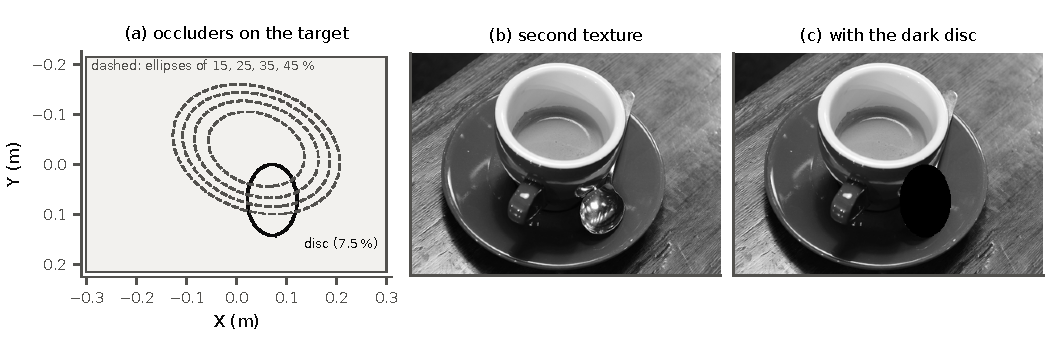
\includegraphics[width=\textwidth]{figures/fig_scenes.pdf}
\caption{Scenes. (a) Occluders on the target plane: the disc of the
confirmatory campaign and the replication (7.5\,\% of the image at the desired
pose), and the four ellipses of the sweep. (b) The second texture, clean, and
(c) with the dark disc. \todo{add the reference texture of~\cite{herpvs} as a
panel, subject to its licence.}}
\label{fig:scenes}
\end{figure}

\subsection{Outcomes}
The pose error is that of the camera, the relative pose
${}^{c^{*}}\mathbf{M}_{c}$. The final camera-centre error (mm) and rotation
error (deg) are the medians over the last 50 iterations.\footnote{The
translation of the target frame seen from the camera,
$\mathbf{t}({}^{c}\mathbf{M}_{o})-\mathbf{t}({}^{c^{*}}\mathbf{M}_{o})$, barely
changes when the camera rotates about the target and understates the
camera-centre error by about $Z\theta$: for a run that ends 175\,mm from the
desired camera position it reports 17\,mm.} A run is a \emph{success} if both
errors are below 20\,mm and 1$^{\circ}$. These thresholds were fixed after
the pilot, where they separated converged runs (below 17\,mm and
0.71$^{\circ}$) from basin failures (above 440\,mm and 19$^{\circ}$). A
\emph{basin failure} is a run ending with a rotation error above 5$^{\circ}$; it
distinguishes a wrong basin from the occlusion bias of the unweighted scheme.
Each run also logs, at every iteration, the rank margin
$\lambda_{\min}(\HW)/(\tr(\HW)/6)$, the fraction of weights below 0.25 and
the time spent computing the weights.

\subsection{Statistical analysis}
The unit of analysis is the initial pose, and every comparison between two
weightings is paired over poses. The effect of A against B is the
Hodges--Lehmann estimate~\cite{hodges1963} of the median of the per-pose
log-ratios, back-transformed to a ratio A/B, with its exact distribution-free
95\,\% confidence interval from the Walsh averages. The test is the two-sided
Wilcoxon signed-rank test~\cite{wilcoxon1945}, exact for $n\le50$. Accuracy
comparisons of the pre-registered families are made over the poses where both
runs succeed, so that a basin failure does not enter an accuracy comparison. A test
requires at least six such poses. Success is compared with the exact McNemar
test~\cite{mcnemar1947} on paired indicators, and success rates are reported
with Clopper--Pearson intervals~\cite{clopper1934}. Equivalence within
$\pm25\,\%$ is declared when the 95\,\% CI of the ratio lies in $[0.8,1.25]$,
which is a two-one-sided test~\cite{schuirmann1987tost} at 5\,\% per outcome.
Multiplicity is controlled with Holm's procedure~\cite{holm1979} within each
pre-registered family. Secondary comparisons are reported with their exact
95\,\% CIs. These intervals are not adjusted for multiplicity and carry no
confirmatory weight.

\subsection{Pre-registration and design}
\label{sec:prereg}
A pilot of 160 runs on the four development poses fixed the success
thresholds and the hypotheses. It also led to dropping the adaptive-floor
weighting, which showed no consistent effect. The confirmatory pre-registration
was then committed to the project repository before the first confirmatory
run; an addendum for the replication and the sweep was committed before
either was run. Table~\ref{tab:design} summarises the three campaigns.

\begin{table}[t]
\centering
\caption{Design. All runs: 32 initial poses, 600 iterations, both interaction
matrices.}
\label{tab:design}
\small
\begin{tabular}{@{}llp{0.52\textwidth}r@{}}
\toprule
Campaign & Weightings & Scenes & Runs \\
\midrule
Confirmatory & V1--V4 & reference texture: clean; disc dark, textured, low-contrast & 1\,024 \\
Replication & V2, V3 & second texture: clean; disc dark & 256 \\
Sweep & V2, V3 & reference texture: dark ellipse, $f=15,25,35,45\,\%$ & 512 \\
\bottomrule
\end{tabular}
\end{table}

The confirmatory primary family comprises six tests, Holm-corrected together:
\begin{itemize}
\item \textbf{P1a, P1b}: V3 against V2, desired-image matrix, dark disc,
  camera-centre and rotation error. Prediction: V3 more accurate.
\item \textbf{P2a--d}: success of V3 against V2 with the current-image matrix,
  in each of the four scenes. Prediction, from the pilot: V3 succeeds less
  often.
\end{itemize}
The decision rule was fixed with them. If P1a and P1b are both significant with
a median ratio of at most 0.8, the study is reported as a method paper on V3;
otherwise as an analysis paper. The replication family (R1a, R1b) repeats P1a
and P1b on the second texture, with the same criterion. The sweep family
(S, 24 tests) comprises V3 against V2 on both errors (16 tests) and on
success (8 tests), in each combination of fraction and matrix.

\subsection{Reproducibility}
The servoing program, the pose and occluder generators, the run scripts, the
analysis program with its end-to-end self-test on synthetic data, the
per-iteration logs and the pre-registration documents with their commit
history are available at \todo{repository URL and archive DOI}. The reference
texture cannot be redistributed; the second texture is in the public domain.

% =====================================================================
\section{Results}
\label{sec:results}

\subsection{Primary family}

Table~\ref{tab:primary} gives the six pre-registered tests. Both accuracy tests
are significant after Holm with a median ratio of 0.66, below the 0.8
threshold, so the pre-registered decision is a method paper. None of the four
success tests is significant: with the current-image matrix and the 7.5\,\%
disc, V3 and V2 converge from similar numbers of poses (26--27 against 28--31
of 32).

\begin{table}[t]
\centering
\caption{Pre-registered primary family (Holm over six tests). Ratios are
Hodges--Lehmann estimates of V3/V2 with exact 95\,\% CIs, over the poses where
both succeed.}
\label{tab:primary}
\small
\resizebox{\textwidth}{!}{%
\begin{tabular}{@{}llllr@{}}
\toprule
Test & Comparison & Result & $p$ (Holm) & Verdict \\
\midrule
P1a & camera-centre error, $\mathbf{L}(I^{*})$, dark disc & 0.658 [0.600, 0.732], $n=29$ & $4.2\times10^{-7}$ & supported \\
P1b & rotation error, same & 0.657 [0.600, 0.732], $n=29$ & $4.2\times10^{-7}$ & supported \\
P2a & success, $\mathbf{L}(I)$, clean & V3-only 2, V2-only 5 & 1 & not supported \\
P2b & success, $\mathbf{L}(I)$, dark disc & V3-only 2, V2-only 3 & 1 & not supported \\
P2c & success, $\mathbf{L}(I)$, textured disc & V3-only 2, V2-only 3 & 1 & not supported \\
P2d & success, $\mathbf{L}(I)$, low-contrast disc & V3-only 1, V2-only 6 & 0.50 & not supported \\
\bottomrule
\end{tabular}}
\end{table}

\subsection{Accuracy}

Table~\ref{tab:accuracy} gives the final errors and success counts of the
confirmatory campaign, and Fig.~\ref{fig:forest} the V3/V2 ratio in every cell
of the study where it can be computed.

\begin{table}[t]
\centering
\caption{Confirmatory campaign: median final camera-centre error (mm) and
rotation error (deg) of the successful runs, and number of successes out of
32. For V1 under the dark and textured discs no run succeeds; the median over
all runs is given in italics.}
\label{tab:accuracy}
\small
\setlength{\tabcolsep}{4pt}
\resizebox{\textwidth}{!}{%
\begin{tabular}{@{}llllll@{}}
\toprule
$\Lh$ & Scene & V1 & V2 & V3 & V4 \\
\midrule
$\mathbf{L}(I)$ & clean & 5.36, 0.238 (30) & 12.4, 0.541 (29) & 7.99, 0.351 (26) & 10.3, 0.451 (26) \\
 & dark disc & \emph{35.5, 1.53} (0) & 0.447, 0.020 (28) & \textbf{0.327, 0.014} (27) & 0.387, 0.017 (23) \\
 & textured disc & \emph{34.8, 1.51} (0) & 0.450, 0.020 (28) & \textbf{0.329, 0.014} (27) & 0.382, 0.017 (25) \\
 & low-contrast disc & 15.7, 0.678 (32) & 0.985, 0.043 (31) & \textbf{0.331, 0.015} (26) & 0.755, 0.033 (26) \\
\midrule
$\mathbf{L}(I^{*})$ & clean & 5.22, 0.230 (31) & 13.4, 0.590 (31) & 8.81, 0.389 (29) & 12.0, 0.527 (32) \\
 & dark disc & \emph{31.6, 1.37} (0) & 0.489, 0.022 (32) & \textbf{0.321, 0.014} (29) & 0.443, 0.019 (32) \\
 & textured disc & \emph{31.3, 1.35} (0) & 0.493, 0.022 (32) & \textbf{0.311, 0.014} (29) & 0.447, 0.020 (32) \\
 & low-contrast disc & 15.0, 0.649 (31) & 0.939, 0.041 (32) & \textbf{0.351, 0.015} (29) & 0.894, 0.039 (32) \\
\bottomrule
\end{tabular}}
\end{table}

\begin{figure}[t]
\centering
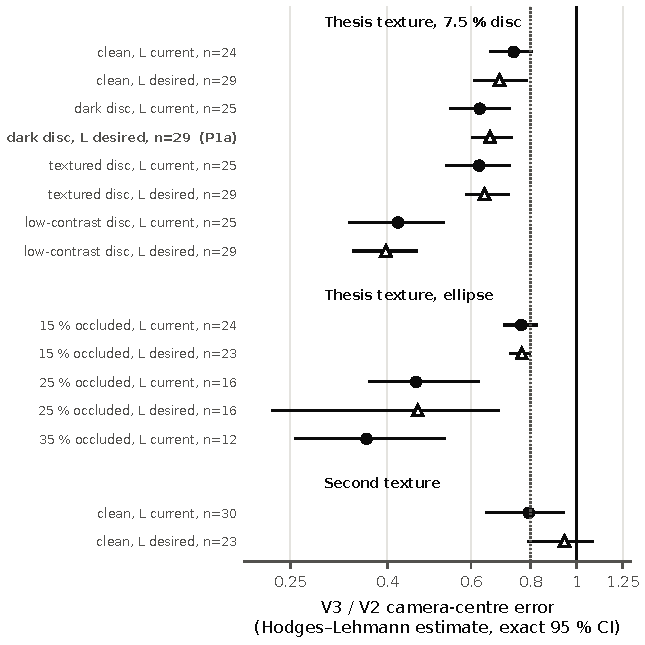
\includegraphics[width=0.62\textwidth]{figures/fig_forest.pdf}
\caption{V3/V2 final camera-centre error over the poses where both succeed, in
every cell where at least six such poses exist. Filled circles: current-image
matrix; open triangles: desired-image matrix. The bold row is the
pre-registered test P1a. The dotted line marks the 0.8 threshold of the
decision rule. Missing cells: the occluded second texture (V2 never succeeds),
the sweep at 45\,\% (no successes for V3 with $\mathbf{L}(I)$ or for V2 with
$\mathbf{L}(I^{*})$) and at 35\,\% with $\mathbf{L}(I^{*})$ (five pairs). The
rotation error gives the same ratios to two decimals.}
\label{fig:forest}
\end{figure}

\paragraph{Robust weighting removes the occlusion bias}
Without weighting, the camera converges to a pose 31--35\,mm and
1.35--1.53$^{\circ}$ from the target under the dark and textured discs. With
V2 the error falls by a factor of about 65 (V2/V1 over all poses:
0.015, 95\,\% CI 0.012--0.020). The low-contrast disc biases V1 less
(15.0--15.7\,mm), within the success threshold, and V2 reduces that bias by a
factor of 16. On the clean scene robustness has a cost: V2 is 2.4--2.5 times
less accurate than V1 (CI 2.00--2.78), because the estimator rejects valid
textured measurements while the pose error is large.

\paragraph{V3 is more accurate than V2 at iteration 600 in every cell}
Where both converge, V3 reduces V2's final error in all eight confirmatory
cells (Fig.~\ref{fig:forest}). The reduction is largest under the low-contrast
disc (ratios 0.40--0.42), about a third under the dark and textured discs
(0.62--0.66) and a quarter to a third on the clean scene (0.69--0.74). It holds
with both interaction matrices. On the clean scene V3 remains 1.5--1.7 times
less accurate than V1. The structure-penalised weighting V4 lies between: its
ratio to V2 is 0.89--0.94, equivalent within $\pm25\,\%$ in six of the eight
cells.

\paragraph{The gain at iteration 600 grows with the occluded fraction}
In the sweep, V3/V2 where both succeed is 0.77 at 15\,\% occlusion with either
matrix (95\,\% CIs 0.70--0.83 and 0.72--0.80), 0.46 at 25\,\% (0.36--0.62 and
0.23--0.69) and 0.36 at 35\,\% with the current-image matrix (0.25--0.53), all
significant after Holm within family S ($p\le0.003$). Three cells of the family
cannot be tested (Fig.~\ref{fig:forest}), so its pre-specified statement that
the gain holds at every fraction is not met. On the clean second texture the
gain is smaller and not significant: 0.79 (0.64--0.94) with the current-image
matrix and 0.94 (0.79--1.09) with the desired-image matrix.

\paragraph{The advantage depends on the iteration budget (exploratory)}
The pre-registered outcome is the error at a fixed budget of 600 iterations
(24\,s of simulated time). Figure~\ref{fig:budget} shows the median per-pose
ratio V3/V2 at earlier budgets. Under the dark and textured discs it rises from
0.09--0.19 at iteration 100 to 0.39--0.44 at 300 and 0.62--0.64 at 600, and it
is still rising at the end: between iterations 300 and 600, V2 halves its
error (median factor 0.52--0.57) while V3 reduces it by only 12--15\,\%. The
same holds in every occluded cell of the sweep (at 25\,\% with the
current-image matrix, 0.15 at iteration 300 and 0.52 at 600). On the clean
scene the ratio levels off at 0.67 (desired-image matrix) and 0.74--0.77
(current-image matrix). V3 therefore reaches a given accuracy sooner, and the
larger gains at larger occluded fractions reflect at least in part the slower
convergence of V2. Whether V3's error at convergence is also smaller cannot be
decided from runs of this length.

\begin{figure}[t]
\centering
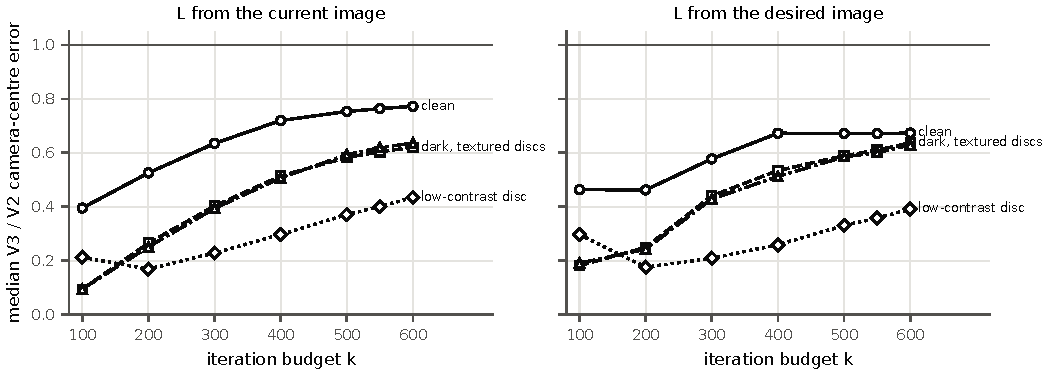
\includegraphics[width=\textwidth]{figures/fig_budget.pdf}
\caption{Median over the poses where both succeed of the per-pose ratio of
V3's to V2's camera-centre error, at iteration $k$ (each error the median over
the 25 iterations up to $k$); confirmatory campaign. The dark and textured
discs give nearly identical curves.}
\label{fig:budget}
\end{figure}

\subsection{Convergence}

\begin{figure}[t]
\centering
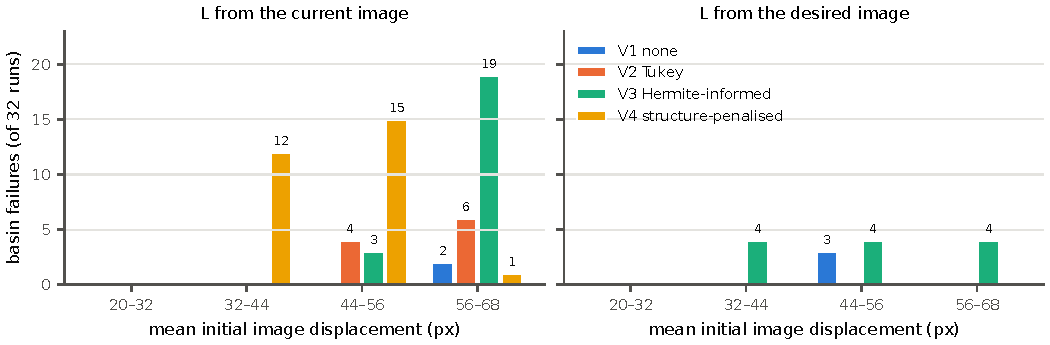
\includegraphics[width=\textwidth]{figures/fig_basin.pdf}
\caption{Basin failures (final rotation error above 5$^{\circ}$) in the
confirmatory campaign, by bin of initial image displacement; 32 runs per bin
and weighting (eight poses, four scenes).}
\label{fig:basin}
\end{figure}

Figure~\ref{fig:basin} shows where the basin failures occur. With the
current-image matrix, V3 fails from 19 of the 32 runs of the largest
displacement bin and from none below 44\,px; V4 fails at intermediate
displacements (12 and 15 of 32 in bins 1 and 2); V2 fails from 10 of the 64 runs
in the two largest bins. With the desired-image matrix, V2 and V4 never fail
and V3 fails from three poses (poses 13, 24 and 27, in every scene). The
current-image matrix thus narrows the convergence domain of the
structure-based weightings, each at its own range of displacements, while the
desired-image matrix, despite being exact only at the desired pose, lets V2 and
V4 converge from every pose tested, at displacements up to 58\,px.

\begin{figure}[t]
\centering
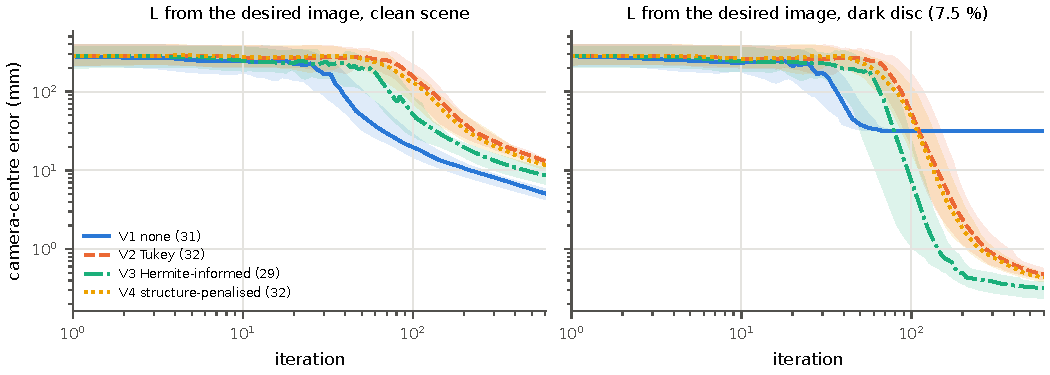
\includegraphics[width=\textwidth]{figures/fig_curves.pdf}
\caption{Median (line) and interquartile range (band) of the camera-centre
error over the successful runs, desired-image matrix; the number of runs is
given in the legend. On the clean scene the error decays algebraically. Under
the disc V1 reaches a stationary biased pose, while the weighted schemes are
still converging at iteration 600.}
\label{fig:curves}
\end{figure}

\paragraph{Algebraic decay on the clean scene}
Figure~\ref{fig:curves} shows the two regimes of
Proposition~\ref{prop:rate}. On the clean scene the error decays
algebraically: the median slope of $\log\lVert\Delta\mathbf{t}\rVert$ against
$\log k$ over $k\ge200$ is $-0.63$ to $-0.66$ for V1 and V3 and $-0.73$ to
$-0.93$ for V2 and V4. That is steeper than the $-1/2$ of the idealised
analysis, but it is not geometric, and the error is still decreasing at the
last iteration. Under the dark and textured discs the weighted runs end within
0.3--0.5\,mm of the target, more than an order of magnitude closer than on the
clean scene, because the occlusion residual keeps the gain finite. V1 reaches a
stationary biased pose, as Proposition~\ref{prop:rate} predicts for fixed
weights. The weighted runs are not stationary: their weights change as the
robust scale contracts, which moves the equilibrium of the weighted law, and
the error keeps decreasing algebraically (median slope $-1.0$ to $-1.3$ for
V2, $-0.25$ to $-0.33$ for V3). The geometric regime of
Proposition~\ref{prop:rate}, which assumes fixed weights, is therefore observed
only for V1. In both scenes the final error is a property of the iteration
budget as well as of the estimator.

\subsection{Replication on a second texture}

\begin{table}[t]
\centering
\caption{Replication on the second texture: successes out of 32, and median
final errors (camera centre, rotation). For V2 under the disc the median is
over all runs (no success). McNemar $p$ values are Holm-adjusted within the
replication family.}
\label{tab:replication}
\small
\resizebox{\textwidth}{!}{%
\begin{tabular}{@{}lllllr@{}}
\toprule
$\Lh$ & Scene & V2 & V3 & V3-only / V2-only & $p$ (Holm) \\
\midrule
$\mathbf{L}(I)$ & clean & 10.0\,mm, 0.440$^{\circ}$ (32) & 8.57\,mm, 0.377$^{\circ}$ (30) & 0 / 2 & 0.50 \\
 & dark disc & \emph{128.1\,mm, 5.62$^{\circ}$} (0) & 6.63\,mm, 0.298$^{\circ}$ (24) & 24 / 0 & $3.6\times10^{-7}$ \\
$\mathbf{L}(I^{*})$ & clean & 9.97\,mm, 0.438$^{\circ}$ (31) & 8.71\,mm, 0.383$^{\circ}$ (24) & 1 / 8 & 0.078 \\
 & dark disc & \emph{174.8\,mm, 7.69$^{\circ}$} (0) & 8.36\,mm, 0.363$^{\circ}$ (28) & 28 / 0 & $3.0\times10^{-8}$ \\
\bottomrule
\end{tabular}}
\end{table}

Table~\ref{tab:replication} gives the replication. The pre-registered tests
R1a and R1b cannot be computed. Under the dark disc, V2 succeeds from none of
the 32 poses with either matrix, so no pose has both runs successful. By the
pre-registered criterion the primary result is therefore \emph{not
replicated}. The reason, however, is a failure of the reference method, not of
V3. The pre-registered secondary success tests show V3 converging where V2
does not: from 28 against 0 poses with the desired-image matrix
($p=3.0\times10^{-8}$) and from 24 against 0 with the current-image matrix
($p=3.6\times10^{-7}$).

The following analysis is exploratory. V2 reaches the same final pose from every
initial pose: the interquartile range of its camera-centre error is
127.7--128.3\,mm with the current-image matrix and 174.7--174.9\,mm with the
desired-image matrix. It is an equilibrium of the weighted law, not a basin
failure. From pose 1 the trajectory passes within 42\,mm of the target at
iteration 144 and then moves away. The offset is
$\Delta\mathbf{t}=(-19.6,\,171.3,\,28.5)$\,mm with
$\theta\mathbf{u}=(7.63,\,0.88,\,-0.10)^{\circ}$: a translation along $y$
coupled with a rotation about $x$, $\Delta t_{y}\approx Z^{*}\theta_{x}$. Along
this direction the image of a fronto-parallel plane changes only at second
order~\cite{chaumette1998potential}. From the same pose, the unweighted law ends
78\,mm from the target and V3 8.4\,mm, so V2 ends farther away than no
weighting at all, and at a higher final cost ($4.62\times10^{10}$ against
$4.02\times10^{10}$ and $3.98\times10^{10}$). Started at the desired pose,
every weighting drifts away along the same direction, so the desired pose is
not an equilibrium under this occlusion.

Figure~\ref{fig:maps} locates the cause. At V2's final pose, Tukey's estimator
rejects most of the disc but keeps a curved band inside it. In that band the
hidden texture, the shadowed handle of the cup, is about as dark as the
occluder, so the residual falls within the estimator's acceptance region. With
the desired-image matrix these measurements have the non-zero rows of the
hidden texture (Proposition~\ref{prop:inert}), and they carry the influence that
remains inside the occluder. V3 rejects the whole disc: $\Gb$ is computed from
the current image, which is uniform inside the disc, so every non-zero residual
there is divided by the floor and rejected. V3 thus identifies the occluder by
its lack of structure, whether or not its grey level happens to match the
texture it hides. With the current-image matrix the interior of the disc has
zero rows, so V2's equilibrium in that case (128\,mm, in the same direction)
must arise from the boundary band; maps were not recorded for it. V3 is not
free of bias on this texture either: it converges to 6.6--8.4\,mm, against
0.33\,mm on the reference texture.

\begin{figure}[t]
\centering
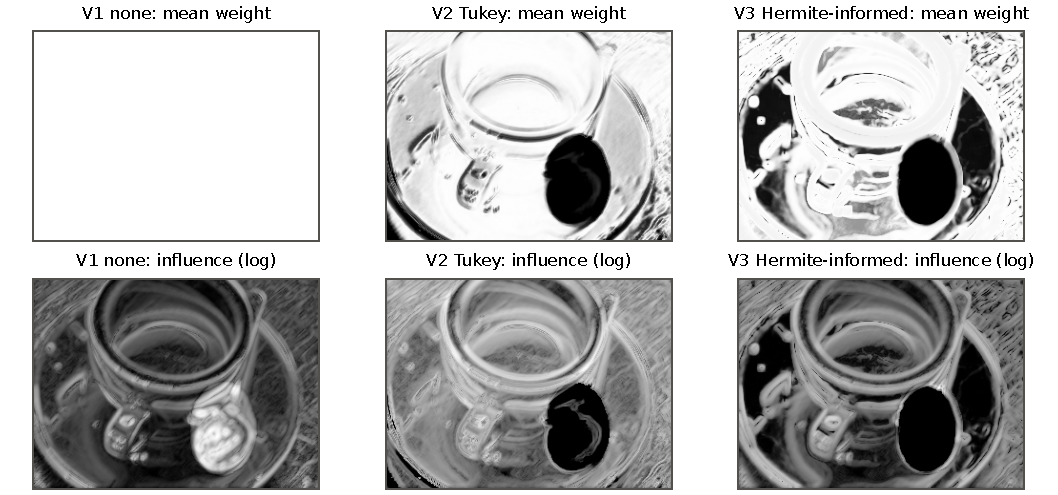
\includegraphics[width=\textwidth]{figures/fig_maps.pdf}
\caption{Second texture, dark disc, desired-image matrix, pose 1, final
iteration. Top: weight averaged over the four channels at each position (white
1, black 0). Bottom: influence $\sum_{k}\lVert w_{j}\boldsymbol{\ell}_{j}\rVert\,\lvert w_{j}e_{j}\rvert$
per position, logarithmic. V2 keeps a band of measurements inside the disc, where the
hidden texture is dark; V3 rejects the whole disc.}
\label{fig:maps}
\end{figure}

\subsection{Occluded fraction}

\begin{table}[t]
\centering
\caption{Sweep: successes out of 32. The 7.5\,\% row is the confirmatory dark
disc, for reference. McNemar $p$ values are Holm-adjusted within family S
(24 tests).}
\label{tab:sweep}
\small
\begin{tabular}{@{}lrrlrrrl@{}}
\toprule
 & \multicolumn{3}{c}{$\mathbf{L}(I)$} & & \multicolumn{3}{c}{$\mathbf{L}(I^{*})$} \\
\cmidrule{2-4}\cmidrule{6-8}
$f$ & V2 & V3 & $p$ & & V2 & V3 & $p$ \\
\midrule
7.5\,\% & 28 & 27 & -- & & 32 & 29 & -- \\
15\,\% & 27 & 24 & 0.50 & & 27 & 27 & 1 \\
25\,\% & 28 & 16 & 0.0029 & & 16 & 30 & $8.5\times10^{-4}$ \\
35\,\% & 25 & 14 & 0.022 & & 5 & 28 & $4.1\times10^{-6}$ \\
45\,\% & 20 & \textbf{0} & $2.7\times10^{-5}$ & & \textbf{0} & 27 & $2.7\times10^{-7}$ \\
\bottomrule
\end{tabular}
\end{table}

\begin{figure}[t]
\centering
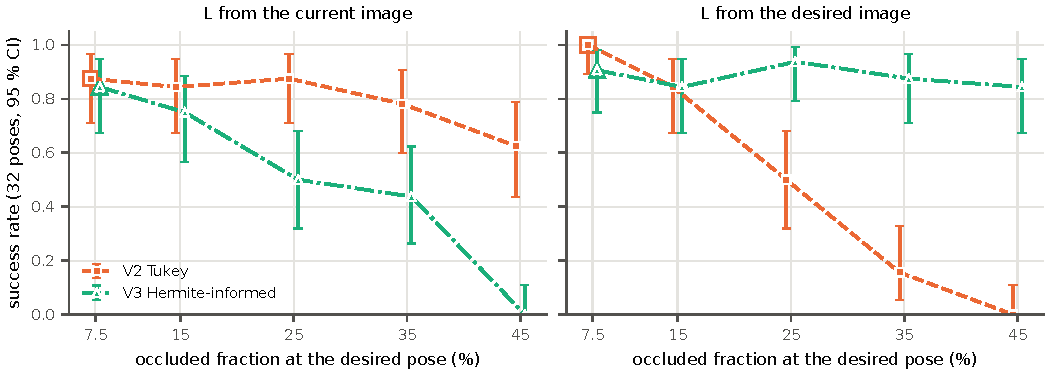
\includegraphics[width=\textwidth]{figures/fig_sweep.pdf}
\caption{Success rate against the occluded fraction at the desired pose, with
Clopper--Pearson 95\,\% intervals. The larger marker at 7.5\,\% is the
confirmatory disc. The ordering of V2 and V3 reverses with the interaction
matrix.}
\label{fig:sweep}
\end{figure}

Table~\ref{tab:sweep} and Fig.~\ref{fig:sweep} give the sweep. The two
weightings break down in opposite configurations. With the desired-image
matrix, V3 converges from 27--30 of 32 poses at every fraction up to 45\,\%,
while V2 falls to 16 at 25\,\%, 5 at 35\,\% and 0 at 45\,\%. With the
current-image matrix, V2 retains 20 of 32 at 45\,\% while V3 falls to 16, 14
and 0. The differences at 25, 35 and 45\,\% are significant after Holm in both
configurations. The failures are divergences, not biased equilibria: 168 of
the 198 failed runs are still moving at the last iteration, and they end
68\,mm to 4.7\,m and 3--175$^{\circ}$ from the target. Successful runs become
\emph{more} accurate at iteration 600 as the fraction grows (V3 with the
desired-image matrix: 0.33, 0.23, 0.11 and 0.02\,mm), consistent with a gain
that the persistent residual keeps finite (Proposition~\ref{prop:rate}).

The two failure modes differ; the following diagnostics are exploratory. With
the desired-image matrix, V2 rejects too little. At the first iteration it
gives a weight below 0.25 to only 4--10\,\% of the measurements, whereas the
occluder covers 17--73\,\% of the image. At pose 1 and $f=45\,\%$, its mean
weight inside the occluder is 0.73, and the occluder's interior carries 55\,\%
of the total influence on the control (V3: weight 0.36, influence 9\,\%). With
the current-image matrix the same interior carries 4\,\% of the influence, as
Proposition~\ref{prop:inert} requires, and V2 converges. V3 with the
current-image matrix fails late. At pose 1 and $f=45\,\%$ it comes within
75\,mm of the target at iteration 100, then moves away along the weakly
observable direction ($\Delta t_{y}/\theta_{x}=1.29$\,m), reaching 1.1\,m and
51$^{\circ}$ at iteration 600, while the unweighted feature cost
\emph{decreases} ($3.46\times10^{11}$ to $3.38\times10^{11}$ between iterations
100 and 150). Its success rate falls both with the initial coverage (0.79
below 20\,\%, 0.09 above 50\,\%) and with the displacement bin (0.59 to 0.16).
The mechanism of this failure is not established.

\subsection{Further measurements}

\paragraph{Stability margin}
The rank margin $\lambda_{\min}(\HW)/(\tr(\HW)/6)$ never fell below
$5.8\times10^{-6}$ in any of the 1\,792 runs, so no failure is a loss of rank.
The bound $\delta_{\W}$ of~\eqref{eq:deltaW}, evaluated with
$\max_{i}(\HW)_{ii}\le\tr\HW$, is at most 0.10 over the last 50 iterations of
every successful confirmatory run and at most 0.42 in the replication, so the
sufficient condition of Proposition~\ref{prop:reweighting} holds there. In
the sweep the persistent residual keeps $\mu$ large, and the bound (median 57)
is not informative.

\paragraph{The final cost does not rank accuracy under occlusion}
Within a pose, Kendall's $\tau$ between the final feature cost
$\lVert\e\rVert^{2}$ and the camera-centre error of the four weightings is
0.83--1.0 on the clean scene. Under the three occluders with the
desired-image matrix it is $-0.33$ to $-0.67$, negative at 72--84\,\% of the
poses. A lower final cost then indicates a \emph{less} accurate pose, so the
cost cannot serve to select a weighting or to declare convergence.

\paragraph{Cost of the weights}
Per iteration, the weights take 10.5\,ms for V2, 12.7\,ms for V3 and 11.7\,ms
for V4 (medians), against 239\,ms for a whole iteration of the unoptimised
program. The structure measure of V3 adds 2.2\,ms, under 1\,\% of an
iteration.

% =====================================================================
\section{Discussion}
\label{sec:discussion}

\paragraph{Two ways to fail}
The results fit one account. A residual-based estimator rejects a measurement
when its residual is large. An occluder's measurements do not always have large
residuals: where the hidden texture is close to the occluder in grey level,
they pass the test. Whether these surviving measurements matter depends on the
interaction matrix. With the current-image matrix, the interior of a uniform
occluder has zero rows (Proposition~\ref{prop:inert}), so the retained
measurements exert no force and V2 converges even at 45\,\% occlusion. With
the desired-image matrix they have the rows of the hidden texture. They then
bias the equilibrium, along the weakly observable translation--rotation
direction on the second texture, or cause divergence when the occluder is
large. The structure-informed weighting removes this failure because it judges
a measurement by the presence of structure in the current image, which an
untextured occluder lacks whatever its grey level. Its own failure lies
elsewhere: with the current-image matrix and a large occluder, the
structure-informed weighting first approaches the target and then leaves it
along the weakly observable direction. We have not established why. The
evidence---a late departure while the unweighted cost decreases, more frequent
at large displacements and large coverages---points to a weighted cost that
has a spurious minimum along that direction, but it does not prove it.

\paragraph{Practical consequence}
No weighting is robust under both interaction matrices. Within the conditions
tested, V3 with the desired-image matrix is the only configuration that
withstands both a large occluder (no breakdown up to 45\,\%) and the second
texture (28 of 32 poses), and at a budget of 600 iterations it is the most
accurate configuration whenever it converges. Its price is a smaller convergence domain on a clean scene: it
fails from 3 of 32 poses on the reference texture and 8 of 32 on the second
one, against 1 for V2 with the same matrix (not significant after Holm). With
the current-image matrix, V2 is the safer choice for large occluders, at the
cost of accuracy. The interaction matrix should therefore be chosen together
with the weighting, not separately.

\paragraph{What the pre-registration changed}
Three findings contradicted expectations formed before the confirmatory data.
Proposition~\ref{prop:inert} suggested that, with the current-image matrix and
a uniform occluder, V3 could not outperform V2, since the weights on the
occluder's interior are inert. Yet V3 is more accurate in that configuration
(0.63, 0.54--0.73): its gain comes through the textured measurements, which is
also why it appears on the clean scene. The pilot suggested a large convergence
penalty for V3 with the current-image matrix (two of four poses lost). The
confirmatory campaign shows a penalty confined to the largest displacements,
and P2 was not supported. The replication, designed to repeat P1, failed for an
unanticipated reason that turned out to be the most informative result of the
study. Finally, the pre-registered outcome, the error at a fixed budget,
conflates speed and final bias. We did not anticipate this, and the
exploratory analysis of Fig.~\ref{fig:budget} shows that it matters. Had the analyses been chosen after the data, the first two
points would likely have been reported differently.

\paragraph{Limitations}
The study is a simulation. The rendering is noise-free and identical for the
desired and current images, the illumination is constant, and the target is a
planar texture at a known constant depth, for which the interaction
matrix~\eqref{eq:hermite-row} is exact at the desired pose. The occluders are
painted on the target. A real occluder in front of the target would add
parallax, and its texture would move differently from the target's. Two
textures do not span the variety of real scenes. The second texture showed that
the behaviour of V2 under occlusion depends on the texture the occluder hides,
so the size of the effects reported here should not be extrapolated to other
scenes. The weightings compared are Tukey-based; other influence functions,
leverage-based design weights and learned weights were not studied. The gain
law~\eqref{eq:gains} is that of the scheme under study and shapes the
clean-scene accuracy at a fixed iteration budget. The runs stop after 600 iterations, before
the weighted schemes have converged under occlusion, so the comparison of
final biases at convergence requires longer runs. Finally, the diagnostic
analyses of failures are exploratory and rest on few runs.

% =====================================================================
\section{Conclusion}
\label{sec:conclusion}

In photometric visual servoing with a weighted Levenberg--Marquardt law, the
interaction matrix decides where a robust weighting can act: with the
current-image matrix, weights on untextured regions are inert. A
structure-informed Tukey weighting, which normalises each residual by a
Gauss--Hermite gradient magnitude of the current image, reduces the
positioning error of Tukey weighting after 600 iterations by a third in a
pre-registered comparison (ratio 0.66, $p_{\mathrm{Holm}}=4.2\times10^{-7}$).
The advantage is largest early in the servo and shrinks as the budget grows,
so it is at least partly an advantage in speed. Paired with the desired-image
interaction matrix, it is the only configuration tested that converges from
most initial poses both up to 45\,\% occlusion and on a second texture, where
Tukey weighting converges to a biased equilibrium 175\,mm from the target from
every pose. Residual-based rejection fails when an occluder resembles the
texture it hides. Structure-based rejection does not depend on that
resemblance, but with the current-image matrix it fails at large occlusion
along the weakly observable direction. Longer runs, to compare the biases
at convergence, validation on a robot with physical occluders, and an
explanation of that last failure are the next steps.

\section*{Data availability}
Code, per-run logs and analysis outputs: \todo{repository URL and archive DOI}.

\section*{Declaration of competing interest}
\todo{The authors declare that they have no known competing financial
interests or personal relationships that could have appeared to influence the
work reported in this paper.}

\section*{Acknowledgements}
\todo{funding and acknowledgements}

\appendix

% =====================================================================
\section{Proofs}
\label{app:proofs}

\paragraph{Proof of Proposition~\ref{prop:inert}}
The luminance row at $q$ is
$\boldsymbol{\ell}_{I}(q)=-\nabla I(q)^{\top}\mathbf{L}_{\mathbf{x}}(q)$,
and by~\eqref{eq:hermite-row}
$\boldsymbol{\ell}_{j}=\sum_{q}D_{k(j)}(q-p_{j})\,\boldsymbol{\ell}_{I}(q)$, the
sum running over the kernel support. If the support of the kernel combined
with that of the discrete gradient operator lies in a region where $I$ is
constant, then $\nabla I(q)=\mathbf{0}$ at every $q$ of the kernel support and
$\boldsymbol{\ell}_{j}=\mathbf{0}$. Measurement $j$ contributes
$w_{j}^{2}e_{j}\boldsymbol{\ell}_{j}^{\top}$ to $\Lh^{\top}\W^{2}\e$ and
$w_{j}^{2}\boldsymbol{\ell}_{j}^{\top}\boldsymbol{\ell}_{j}$ to $\HW$. Both
vanish for every $w_{j}$, and hence so does its contribution to $\varepsilon$
and $\diag(\HW)$. The velocity~\eqref{eq:law} depends on $j$ only through the
other weights, that is, through the median and the MAD
of~\eqref{eq:tukey-arg} and, for V3 and V4, through the mean of $G$. With
$\Lh=\mathbf{L}(I^{*})$ the same computation gives
$\boldsymbol{\ell}_{j}=\sum_{q}D_{k(j)}(q-p_{j})\,\boldsymbol{\ell}_{I^{*}}(q)$,
which vanishes only if $I^{*}$ is also uniform on the support. \qed

\paragraph{Proof of Proposition~\ref{prop:reweighting}}
Write $\mathbf{E}=\mu\,\diag(\HW)+\varepsilon\mathbf{I}_{6}\succeq0$, so that
$\KW=\HW+\mathbf{E}$ and $\KW^{-1}\HW=\mathbf{I}_{6}-\boldsymbol{\Delta}$ with
$\boldsymbol{\Delta}=\KW^{-1}\mathbf{E}$. Since $\KW\succeq\HW$,
$\lVert\KW^{-1}\rVert\le1/\lambda_{\min}(\HW)$, and
$\lVert\boldsymbol{\Delta}\rVert\le\lVert\KW^{-1}\rVert\,\lVert\mathbf{E}\rVert\le\delta_{\W}$.
On an unoccluded scene
$\e=\mathbf{L}^{*}\dr+O(\lVert\dr\rVert^{2})$, with $\mathbf{L}^{*}$ the
interaction matrix at $\mathbf{r}^{*}$, and both choices of $\Lh$ satisfy
$\Lh=\mathbf{L}^{*}+O(\lVert\dr\rVert)$. Hence
$\Lh^{\top}\W^{2}\e=\HW\dr+O(\lVert\dr\rVert^{2})$. The remainder is
multiplied by $\KW^{-1}$, which is bounded when $\lambda_{\min}(\HW)/\tr\HW$ is
bounded away from zero. Then
$\vc=-\lambda(\mathbf{I}_{6}-\boldsymbol{\Delta})\dr+O(\lVert\dr\rVert^{2})$
and
$\dr_{k+1}=\bigl((1-T\lambda_{k})\mathbf{I}_{6}+T\lambda_{k}\boldsymbol{\Delta}_{k}\bigr)\dr_{k}+O(\lVert\dr_{k}\rVert^{2})$.
For $T\lambda_{k}\le1$ the norm of the matrix is at most
$1-T\lambda_{k}+T\lambda_{k}\bar\delta$, which gives~\eqref{eq:contraction}.
No property of the sequence $\W_{k}$ other than $\delta_{\W_{k}}\le\bar\delta$
was used. \qed

\paragraph{Proof of Proposition~\ref{prop:rate}}
With $\boldsymbol{\Delta}_{k}\to\mathbf{0}$, the recursion of the previous proof
becomes $\dr_{k+1}=(1-T\lambda_{k})\dr_{k}+o(\lVert\dr_{k}\rVert)$: the step
is a scalar multiple of the error, which keeps its direction. With
$\lambda_{k}=N_{e}^{0.2}\bar e_{k}=N_{e}^{-0.8}\lVert\e_{I}\rVert^{2}=N_{e}^{-0.8}\rho_{k}(1+o(1))$,
we have $T\lambda_{k}=c\rho_{k}(1+o(1))$ and
$\rho_{k+1}=(1-c\rho_{k})^{2}\rho_{k}(1+o(1))$. Then
$1/\rho_{k+1}=(1/\rho_{k})(1+2c\rho_{k}+O(\rho_{k}^{2}))=1/\rho_{k}+2c+O(\rho_{k})$,
and summing gives $1/\rho_{k}=2ck+o(k)$. Since
$q_{\min}\lVert\dr\rVert^{2}\le\rho\le q_{\max}\lVert\dr\rVert^{2}$ with
$q_{\min},q_{\max}$ the extreme eigenvalues of $\mathbf{Q}$,
$\lVert\dr_{k}\rVert=\Theta(k^{-1/2})$. Under occlusion the same recursion
holds about $\bar{\mathbf{r}}$ with $\lambda_{k}\to\lambda_{\infty}>0$, and
Proposition~\ref{prop:reweighting} gives the geometric factor. \qed

% =====================================================================
\section{Deviations and unplanned analyses}
\label{app:deviations}

\begin{itemize}
\item The study plan initially placed the adaptive-floor weighting in the
  primary family. The pilot showed no consistent effect, and the weighting was
  dropped before the confirmatory pre-registration.
\item The replication tests R1a and R1b could not be computed (no pose with
  both runs successful). They are reported as not replicated, as the
  pre-registered criterion requires.
\item Three cells of the sweep family have fewer than six pairs and no
  $p$ value, as the addendum specifies.
\item The following analyses are exploratory and were not pre-registered:
  basin failures by displacement bin; the seven diagnostic runs on the second
  texture (from the desired pose and from pose 1, with weight and influence
  maps); the four diagnostic runs at 45\,\% occlusion; the stability bound
  $\delta_{\W}$; Kendall's $\tau$ between cost and accuracy; tail slopes; the
dependence of the V3/V2 ratio on the iteration budget.
\end{itemize}

\bibliographystyle{elsarticle-num}
\bibliography{refs}

\end{document}
